\documentclass[11pt,a4paper]{article}

%============================%
%        BASIC PACKAGES      %
%============================%
\usepackage[a4paper,margin=3cm]{geometry}
\usepackage[T1]{fontenc}
\usepackage[utf8]{inputenc}
\usepackage[english]{babel}
\usepackage{lmodern}          % Better serif font
\usepackage{microtype}        % Better spacing and justification
\usepackage{parskip}          % Paragraph spacing instead of indentation
\usepackage{setspace}
\usepackage{hyperref}
\usepackage{datetime}
\newdateformat{monthyear}{\monthname[\THEMONTH] \THEYEAR}
\date{\monthyear\today}
\usepackage{graphicx}
\usepackage{comment}

%============================%
%        HEADINGS            %
%============================%
\usepackage{titlesec}
\renewcommand{\thesection}{\arabic{section}}    %all arabic is standard
\renewcommand{\thesubsection}{\arabic{section}.\arabic{subsection}}

% enumerate settings
\usepackage{enumitem}                           % for the [resume] option
\renewcommand{\theenumi}{\arabic{enumi}}        %options are {arabic, alph, Alph, roman, Roman}
\renewcommand{\theenumii}{\alph{enumii}}
\renewcommand{\theenumiii}{\roman{enumiii}}

%============================%
%        MATHEMATICS         %
%============================%
\usepackage{amsmath,amssymb,amsthm}
\usepackage{dsfont}
\renewcommand{\P}{\mathbb{P}}
\newcommand{\N}{\mathds{N}}
\newcommand{\Z}{\mathds{Z}}
\newcommand{\Q}{\mathds{Q}}
\newcommand{\R}{\mathds{R}}
\newcommand{\C}{\mathds{C}}
\newcommand{\EX}{\mathbb{E}}
\newcommand{\PP}{\mathcal{P}}           % power set
\newcommand{\ndiv}{\nmid}
\newcommand{\eps}{\varepsilon}
\let\temp\phi                           % varphi to phi
\let\phi\varphi
\let\varphi\temp
%different set notations
\newcommand{\sub}{\subset}              % new command to refer to standard notation \subset for standard subset (which might be equal)
\newcommand{\subneq}{\subsetneq}        % new command to refer to standard notation \subsetneq for proper subset (not allowed to be equal)
%\renewcommand{\sub}{\subseteq}         % use \subseteq instead of \subset for standard subset (which might be equal)
%\renewcommand{\subneq}{\subset}        % use \subset instead of \subsetneq for proper subset (which is not allowed to be equal)
%\renewcommand{\setminus}{-}            % use - instead of \ for relative complement of sets
%\renewcommand{\neg}{{\sim}}            % use ~ as negation symbol
\newcommand\norm[1]{\lVert#1\rVert}     % norm with double vertical lines
\newcommand\normx[1]{\Vert#1\Vert}      
\newcommand{\bigO}{\mathcal{O}}         % big O notation

%============================%
%        CODE BLOCKS         %
%============================%
\usepackage{minted}
\usemintedstyle{perldoc}
\setminted[haskell]{
  fontsize=\small,
  baselinestretch=1.05,
  frame=leftline,
  rulecolor=\color{black!70},
  framesep=2mm,
  linenos=false,
  tabsize=2,
  breaklines=true,
  autogobble=true
}

%============================%
%         TITLE INFO         %
%============================%
\title{\textbf{MSO Lab Assignment 2:\\
Programming Learning App}}
\author{Jan Huls (4699610), Arwin Moormans (4965957)}


\begin{document}
\maketitle
\section*{Software Design \& Patterns}
Below you will find a Class diagram to show the structure of the application.

\begin{figure}[htbp]\label{fig:class-diagram}
  \centering
  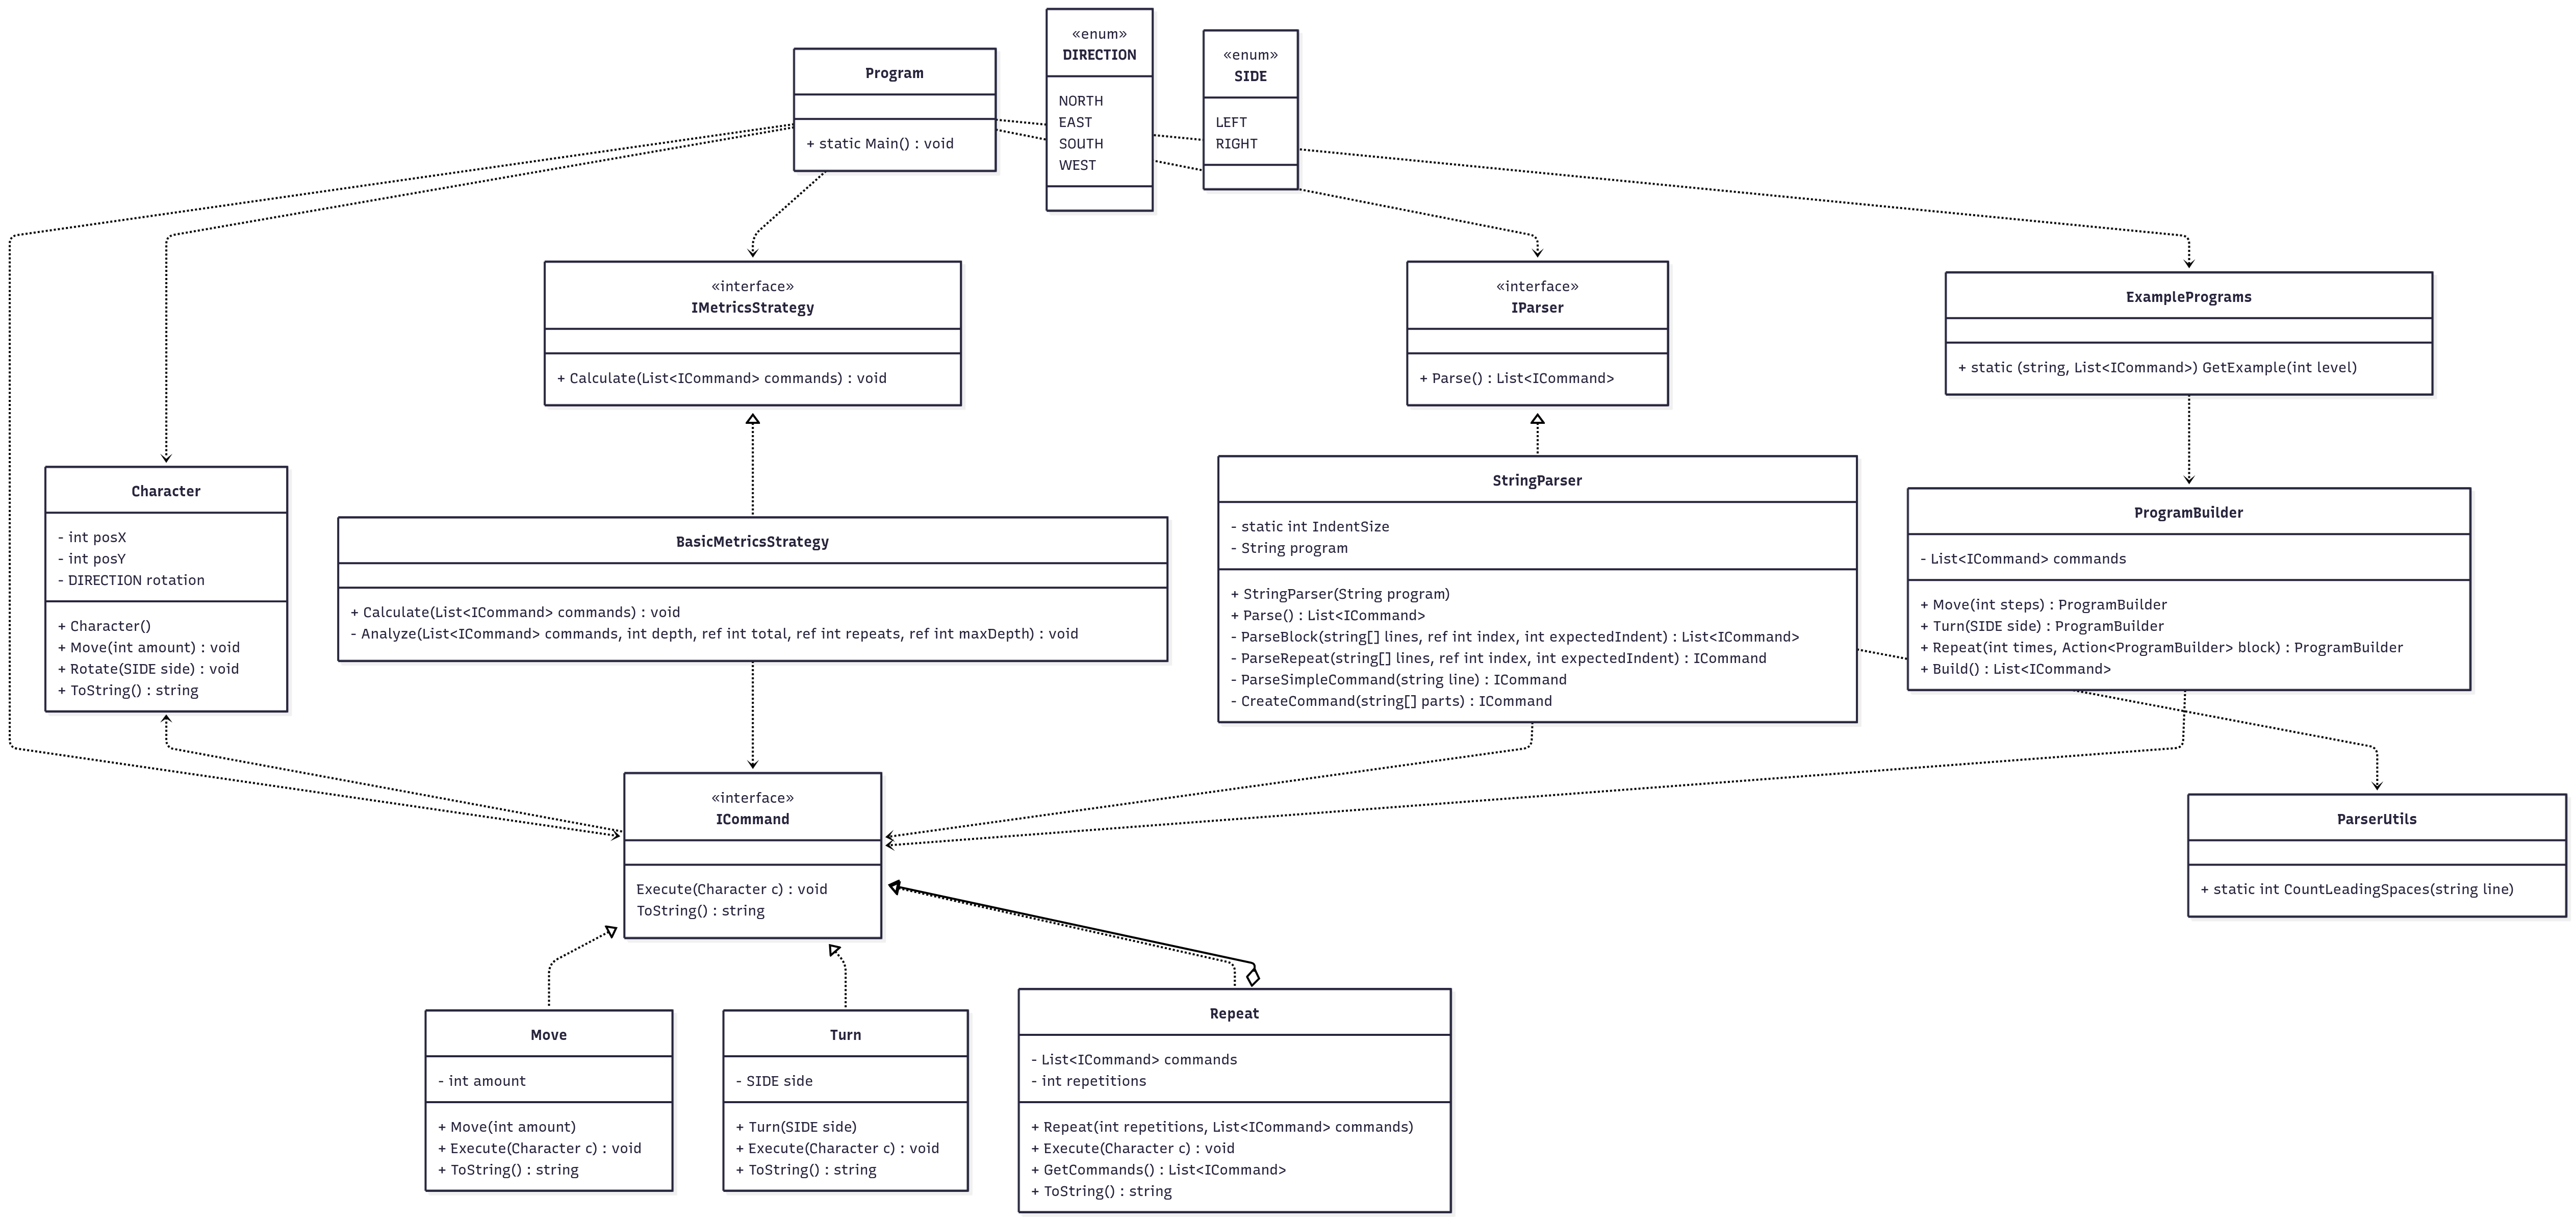
\includegraphics[width=0.9\textwidth]{class_diagram.png}
  \caption{\small{Class diagram of the Programming Learning App}}
\end{figure}
%hier die toevoegen kwee nie hoe da moet
We have used multiple patterns to structure our program. 

The first pattern is the Composite pattern in the repeat command class.
This class holds all the functionality of the repeat command, such as the commands it needs to reapeat and how many times.
Because one of the repeated commands can be another reapeat command, we use the Composite pattern.
This makes a tree like structure where non-repeat commands are leafs and other repeat commands are nodes, meaning \texttt{ICommand} is the component and \texttt{Repeat} is the composite.
This way it is possible to call the Execute function of the root command and that will automaticly execute every command in the tree.

For calculating different metrics we use the Strategy pattern.
This ensures that it is possible to add different kind of metrics later.
By making this a Strategy pattern it is possible to easily change wich kind of metrics the user wants to see.
The IMetricsStrategy is the Strategy interface and the BasicMatricsStrategy is the concrete Strategy.

At last we have used the Builder pattern to create the example programs.
This way it is possible to create 
%mis is deze ook niet nodig?? soort van wrm doen we nii gwn alle commands met de hand aan n lijst toevoegen
% anders moeten we ook deze class aanpassen elke keer als we commando toevoegen
% hmmm, ik denk dat ie wel mooi is zodat iemand die onze code wil implementeren ofz zelf makkelijk voorbeelden kan maken


%Composite pattern bij Repeat
%Strategy pattern bij MetricsCalculator, IMetricsStrategy
%Builder pattern bij ProgramBuilder

\section*{Evaluation}

\begin{comment}
Write an evaluation of your design. First, give an analysis of your design regarding cohesion and cou-
pling. How does your design exhibit high cohesion and low coupling?
Next, explain how your design is capable of handling changing requirements. Identify at least three likely
future changes to the specification. How will your design handle such changes? What kind of changes
would be difficult to incorporate?
\end{comment}

\subsection*{Cohesion}

Our design shows high cohesion in a couple of ways, which we will go through here. 

The \texttt{ICommand} interface is implemented by all the command classes, which all have a single responsibility: executing a specific command. This means that each command class is focused on one task, leading to high cohesion within these classes.
Furthermore, the \texttt{StringParser} class is only responsible for parsing strings from the given format into command objects. This single responsibility ensures that the class is cohesive and easy to maintain.
The \texttt{MetricsCalculator} class is responsible for calculating metrics based on the commands executed. It uses the Strategy pattern to allow for different metric calculation strategies, which keeps the class focused on its core functionality while allowing for flexibility in how metrics are calculated.
The character model in the \texttt{Character} class encapsulates all the properties and behaviors of the character, such as position and direction. This encapsulation ensures that all character-related functionality is contained within a single class, promoting high cohesion.
The \texttt{ProgramBuilder} class is responsible for constructing example programs using the Builder pattern. This class is cohesive as it focuses solely on the creation of program instances, making it easy to understand and modify example programs. 

Overall, our design emphasizes high cohesion by ensuring that each class has a clear and narrow responsibility, making the codebase easier to understand, maintain, and extend.

\subsection*{Coupling}

We demonstrate low coupling in several ways throughout our design. Which we will discuss in this paragraph.

The design uses interfaces such as \texttt{ICommand} and \texttt{IMetricsStrategy} to decouple the implementation of commands and metric strategies from their usage. This allows for easy addition of new commands or metric strategies without affecting existing code, promoting low coupling.
The \texttt{StringParser} class is responsible for parsing input strings into command objects, but it does not depend on the specific implementations of the commands. Instead, it relies on the \texttt{ICommand} interface, which reduces coupling between the parser and command implementations, it does however depend on the concrete command classes to instantiate them, which introduces some level of coupling, but this will always be necessary here, since the parser needs to know which commands to create. 

Overall our program communicates through small interfaces, which reduces dependencies between different parts of the code. This ensures low coupling, making the system more modular and easier to maintain.

\subsection*{Changes}

Here we will discuss $3$ changes which are easy to implement in our program, and one change which is more complex. 

Adding new commands is relatively easy in our design. To add a new command, one would simply need to create a new class that implements the \texttt{ICommand} interface and define the specific behavior for the command in the \texttt{Execute} method. This new command can then be integrated into the existing system without modifying other parts of the code, thanks to the use of interfaces. If this command also needs to be parsed by the \texttt{StringParser}, the parser would need to be updated to recognize the new command string and instantiate the new command class accordingly.

Adding new metric strategies is also straightforward. To introduce a new metric calculation strategy, one would create a new class that implements the \texttt{IMetricsStrategy} interface and define the specific metric calculation logic in the \texttt{Calculate} method. The \texttt{MetricsCalculator} can then utilize this new strategy without any changes to its own implementation, allowing for easy extension of metric calculation capabilities.

Lastly, a new kind of parser could be added, for example to read from a different format. This would involve creating a new parser class that implements the \texttt{IParser} interface. The new parser would handle the specific format and convert it into command objects, similar to how the current parser works. This change would not affect other parts of the system, maintaining low coupling.

A more difficult change would be to implement an undo/redo feature. This would require a change in the \texttt{ICommand} interface to include methods for undoing and redoing commands. Each command class would need to implement these new methods, which could be a lot of work if more commands were added beforehand. Additionally, a new mechanism would need to be introduced to manage the history of executed commands, allowing users to navigate through their command history. This change would involve significant modifications to the existing command structure and could introduce additional complexity in managing command states.

\section*{Work Distribution \& Retrospective}

\begin{comment}
Give a detailed overview of the task distribution: who has worked on which part?
Conduct a retrospective in which you reflect on your collaboration. What went well, and what didn’t?
What should change in upcoming assignments?
\end{comment}

During the project, we divided the work pretty evenly. Both of us have experience with coding, so this made working together easier. 
We liked working together during werkcolleges, as we could discuss ideas and solve problems more efficiently, after which we would both take home tasks to do at home. 
There was not a clear division of tasks since we both worked together a lot, but we both worked on the code and the report. 
We really liked working together, as we could help each other and learn from each other. 
We did not encounter any major issues during the project, but we did have some minor disagreements on how to implement certain features, we were able to resolve these through discussion. 
We have no major changes for upcoming assignments, but we will try to communicate even more effectively to ensure that we are both on the same page.

\end{document}